\documentclass[conference]{IEEEtran}
\usepackage{amsmath,amssymb}
\usepackage{booktabs}
\usepackage{graphicx}
\usepackage{url}
\usepackage{tikz}
\usetikzlibrary{quantikz2,positioning,arrows.meta,fit,backgrounds}
\providecommand{\ket}[1]{\left|#1\right\rangle}
\graphicspath{{../figures/}}

% Project colours (src/bp/style.py): global = vermilion, local = blue
\definecolor{cglobal}{HTML}{E4572E}
\definecolor{clocal}{HTML}{1F77B4}

\newcommand{\Var}{\mathrm{Var}}
\newcommand{\CG}{C_{\mathrm{G}}}
\newcommand{\CL}{C_{\mathrm{L}}}

\begin{document}

\title{Barren Plateaus: Global vs.\ Local Cost Functions}

\author{\IEEEauthorblockN{Saif ur Rehman}
% Add group members here once confirmed.
\IEEEauthorblockA{AI 631 Quantum Machine Learning, Fall 2026 --- Project \#8 (QNN track)\\
Code: \url{https://github.com/Saifix/Barren-plateaus-global-vs.-local-cost-functions}}}

\maketitle

\begin{abstract}
% To be written once all results are in (Week 4).
\emph{Draft, Week~1: introduction and methods only.}
\end{abstract}

% =====================================================================
\section{Introduction}
% =====================================================================
Parameterized quantum circuits (PQCs) trained by gradient descent are the
workhorse of variational quantum algorithms and quantum neural networks. Their
practical value depends on whether they can be trained at all. McClean
\emph{et al.}~\cite{mcclean2018} showed that for sufficiently random circuits
the variance of the cost gradient over random parameters vanishes
exponentially in the number of qubits~$n$. This is called a \emph{barren
plateau}: the landscape is flat almost everywhere, so a gradient must be
estimated to exponential precision, which on a quantum device means an
exponential number of measurement shots~\cite{larocca2025}.

Cerezo \emph{et al.}~\cite{cerezo2021} showed that whether a shallow circuit
has a barren plateau depends on the cost function as well as on the circuit. For
alternating layered ansatzes, a \emph{global} cost, one that compares the
whole $n$-qubit output state with a target, has exponentially vanishing
gradients at any depth. A \emph{local} cost, built from observables that act on
a few qubits, has at worst polynomially vanishing gradients when the depth is
$L=\mathcal{O}(\log n)$. The intuition is a light-cone argument: a local
observable at depth $L$ is affected by only $\mathcal{O}(L)$ neighbouring
qubits, while a global observable is affected by all of them. The link between
locality and trainability was also studied in~\cite{uvarov2021}, and it has since been
characterized exactly for deep circuits through the dynamical Lie
algebra~\cite{ragone2024,fontana2024}. Further work has given general variance
bounds~\cite{zhang2024,letcher2024}, carried the global/local split over to
generative models~\cite{rudolph2024}, and asked whether provable trainability
implies classical simulability~\cite{cerezo2025}. Two further factors matter in
practice. One is initialization: identity blocks~\cite{grant2019},
reduced-domain sampling~\cite{wangqi2024} and classical
initializers~\cite{kashif2024date,kashif2024icrc}. The other is hardware noise,
which can itself flatten the landscape~\cite{wang2021,singkanipa2025} but, if
non-unital, can also protect local costs~\cite{mele2026,sannia2024}.

These results are proved under assumptions, such as local 2-designs or
specific circuit structures, that the circuits people actually train often do not
meet. This project tests the global/local distinction \emph{empirically} on a
hardware-efficient ansatz (HEA) and follows it through to a learning task. We
ask: \emph{how does the gradient variance scale with $n$ and $L$ for a global
and a local cost; does a better initialization help; and how do these effects
appear when training a small classifier, in noise-free simulation, under a
noise model and on IBM hardware?} We test four pre-registered hypotheses, each with an explicit
falsifier (stated in full in the synopsis):
\begin{itemize}
\item[\textbf{H1}] At $L=\lceil\log_2 n\rceil$, $\Var[\partial_k\CG]$ decays
exponentially in $n$ while $\Var[\partial_k\CL]$ decays much more slowly.
\item[\textbf{H2}] For $\CL$, raising the depth from $\lceil\log_2 n\rceil$
to $L\propto n$ makes the variance decay faster.
\item[\textbf{H3}] Identity-block or reduced-domain initialization raises the
initial gradient variance of $\CG$ and speeds up training.
\item[\textbf{H4}] A classifier trained through a global readout learns more
slowly than the same circuit with a local readout, and the gap widens with $n$.
\end{itemize}
Negative results are reported as such.

Our contributions are: (i) a verified, open simulation pipeline that computes
exact gradients for both costs from a single forward/backward pass; (ii) bootstrap
estimates of the variance decay rate for both costs at three depth regimes;
(iii) a leakage-free classification benchmark on fixed folds, with matched
classical baselines, in which the global and local models differ \emph{only} in the
readout; and (iv) noise-model and hardware measurements that separate
cost-induced from noise-induced flattening.

% =====================================================================
\section{Methods}
% =====================================================================

\subsection{Ansatz}
All experiments use the hardware-efficient layered circuit
$V(\boldsymbol\theta)=\prod_{l=1}^{L}W\,\bigotimes_{q=1}^{n}
R_Z(\theta_{l,q,2})R_Y(\theta_{l,q,1})$, where $R_P(t)=e^{-itP/2}$ and $W$
applies CZ gates on qubit pairs $(1,2),(3,4),\dots$ followed by
$(2,3),(4,5),\dots$ (brickwork, Fig.~\ref{fig:circuit}). The circuit has $2nL$
parameters and $(n-1)L$ CZ gates. In the last layer, the $R_Z$ angles are followed
only by diagonal gates and so commute with a $Z$-basis measurement. Their
gradients are therefore identically zero for every cost below. We verify this in
the test suite and exclude these $n$ angles whenever we average over
parameters. This ansatz is \emph{not} guaranteed to satisfy the assumptions
of~\cite{cerezo2021}; testing whether the predicted behaviour holds anyway is
the point of the study.

\begin{figure}[t]
\centering
\resizebox{\columnwidth}{!}{%
\begin{quantikz}[row sep=0.25cm, column sep=0.3cm]
\lstick{$\ket{0}$} & \gate{R_Y(x_1)}
  & \gate{R_Y}\gategroup[wires=4,steps=5,style={dashed,rounded corners,inner sep=3pt},
      label style={label position=below,anchor=north,yshift=-0.15cm}]{one layer, repeated $L$ times}
  & \gate{R_Z} & \ctrl{1} & & & \meter{} \\
\lstick{$\ket{0}$} & \gate{R_Y(x_2)} & \gate{R_Y} & \gate{R_Z} & \control{} & \ctrl{1} & & \meter{} \\
\lstick{$\ket{0}$} & \gate{R_Y(x_3)} & \gate{R_Y} & \gate{R_Z} & \ctrl{1} & \control{} & & \meter{} \\
\lstick{$\ket{0}$} & \gate{R_Y(x_4)} & \gate{R_Y} & \gate{R_Z} & \control{} & & & \meter{}
\end{quantikz}}
\caption{Circuit for $n=4$. Angle encoding $R_Y(x_j)$ (classifier only), then
$L$ HEA layers, then a single $Z$-basis measurement from which both
$\CG$ (all-zeros frequency) and $\CL$ (single-qubit marginals) are computed.}
\label{fig:circuit}
\end{figure}

\subsection{Cost functions}
With $\rho=V(\boldsymbol\theta)\ket{\psi_0}\!\langle\psi_0|V(\boldsymbol\theta)^\dagger$,
\begin{align}
\CG &= 1-\langle 0^{\otimes n}|\rho|0^{\otimes n}\rangle = 1-\langle O_{\mathrm G}\rangle,\\
\CL &= 1-\tfrac{1}{n}\textstyle\sum_{j=1}^{n}\langle 0|\rho_j|0\rangle = 1-\langle O_{\mathrm L}\rangle,
\end{align}
with $O_{\mathrm G}=|0^{\otimes n}\rangle\langle 0^{\otimes n}|$,
$O_{\mathrm L}=\frac1n\sum_j |0\rangle\langle 0|_j\otimes\mathbb 1_{\bar j}$ and
$\rho_j$ the reduced state of qubit $j$, as in~\cite{cerezo2021}. Both
observables are diagonal in the computational basis, so both costs come from the same
measurement record. Both vanish exactly at the solution and are bounded by 1,
so they share the same minimum and range; only their locality differs.

\subsection{Exact gradients}
Because both observables are diagonal, we simulate the circuit with a batched
state-vector simulator (NumPy) and compute all $2nL$ partial derivatives with
the adjoint method~\cite{jones2020}. For each rotation $R_P(\theta_k)$,
$\partial_k\langle O\rangle = \mathrm{Im}\,\langle\lambda_k|P|\phi_k\rangle$,
where $\phi_k$ is the state just after the gate and $\lambda_k$ is $O|\psi\rangle$
propagated back to the same point. One forward and one backward pass give
the full gradient, for either a batch of data points with shared parameters or
a batch of independent parameter draws. The simulator is checked against
Qiskit's \texttt{Statevector} to $10^{-12}$, against central finite differences
and the parameter-shift rule~\cite{schuld2019}, and against the closed-form
variances of the product ansatz $\bigotimes_j R_X(\theta_j)$ on
$\ket{0}^{\otimes n}$,
\begin{equation}
\Var[\partial_1\CG]=\tfrac18\left(\tfrac38\right)^{n-1},\qquad
\Var[\partial_1\CL]=\tfrac{1}{8n^2}
\end{equation}
(Fig.~\ref{fig:analytic}). The global-cost gradient of this ansatz is a product
of $n-1$ independent random factors, so it is heavy-tailed, and its sample
variance converges slowly at large $n$. The test therefore uses a tolerance of
four estimated standard errors rather than a fixed relative tolerance. The same
heavy tail is why every variance below carries a bootstrap interval.

\begin{figure}[t]
\centering
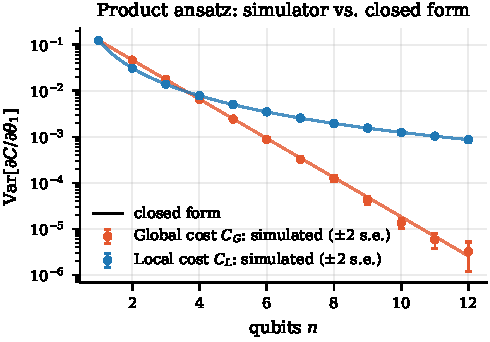
\includegraphics[width=\columnwidth]{analytic_check}
\caption{Validation of the gradient code on the product ansatz: simulated
variances (20\,000 draws, $\pm2$ s.e.) against the closed forms (lines).}
\label{fig:analytic}
\end{figure}

\subsection{Gradient-variance protocol (H1, H2)}
For $n\in\{2,4,\dots,14\}$ and $L\in\{1,\lceil\log_2 n\rceil,n\}$ we draw 200
parameter vectors (2000 for $n\ge10$, see below) $\theta_k\sim U[0,2\pi]$ and compute exact gradients of
$\CG$ and $\CL$ \emph{at the same draws} (a paired comparison), starting from
$\ket{\psi_0}=\ket{0}^{\otimes n}$. We report $\Var[\partial_1 C]$, where
$\theta_1$ is the $R_Y$ angle on qubit 1 in the first layer, and the variance
averaged over all parameters with a non-trivial gradient, each with a 95\%
percentile bootstrap interval (1000 resamples of the draws). The decay rate $b$
is the least-squares slope of $\log\Var = a - b\,n$; its interval comes from
refitting on bootstrap-resampled variances. We use exact rather than sampled
gradients so that the measured quantity is a property of the landscape and not
of the estimator. With $N$ shots, a parameter-shift estimate adds variance
$[p_+(1-p_+)+p_-(1-p_-)]/4N$. For $\CG$ the probabilities are $p_\pm\sim
2^{-n}$, so this term shrinks with $n$ as well and becomes comparable to the
signal at the largest $n$. Finite-shot effects are therefore measured
separately (Sec.~\ref{sec:shots} and~\ref{sec:noise}).

The global-cost gradient is strongly heavy-tailed. In a pilot at $n=14$,
$L=4$, the 5 largest of 1000 draws contributed about 65\% of
$\sum_i(\partial_1\CG)_i^2$, and with 200 draws the 95\% interval for the
variance spanned a factor of 17. We therefore use 2000 draws for $n\ge10$, at
every depth and for both costs (the costs share the same draws).

\subsection{Initializations (H3)}
(i) Uniform, $\theta\sim U[0,2\pi]$; (ii) reduced-domain,
$\theta\sim U[-a,a]$ with $a=\pi/\sqrt{L}$~\cite{wangqi2024}; (iii) identity
blocks~\cite{grant2019}: each block is a random sub-circuit followed by its
adjoint, so it starts as the identity. To keep the identity initialization from
being trivially optimal, the training task prepares
$\ket{\psi_0}=W_0\ket{0}^{\otimes n}$ with a fixed random shallow circuit
$W_0$ and trains $V(\boldsymbol\theta)$ to map it back to
$\ket{0}^{\otimes n}$. Week-1 results use (i) only.

\subsection{Classification task (H4)}
\paragraph*{Data and folds} The Breast Cancer Wisconsin (Diagnostic)
dataset~\cite{street1993}, as shipped with scikit-learn~\cite{pedregosa2011}
(569 samples, 30 features). We take malignant ($212$) as the positive class
$+1$ and benign ($357$) as $-1$, so a majority-class predictor scores $0.627$
accuracy. Following the course NB11 harness, a single stratified 5-fold split
(shuffled, seed 0) is created once, saved to \texttt{data/folds.json} and
used by every model in every table (Fig.~\ref{fig:pipeline}).

\paragraph*{Leakage-free preprocessing} Inside each fold, a standard scaler,
PCA to $n$ components, and a min--max scaler to $[0,\pi]$ are fitted on the
training fold only and then applied to the test fold. Test values outside the
training range are clipped to $[0,\pi]$. A test checks that changing test rows
does not change the fitted transform. We use $n\in\{4,6,8,10\}$ components
(one per qubit) and $L=\lceil\log_2 n\rceil$.

\paragraph*{Quantum model} Features are angle-encoded (Fig.~\ref{fig:circuit}) as
$\ket{\psi_0(\mathbf x)}=\bigotimes_j R_Y(x_j)\ket 0$ and passed through
$V(\boldsymbol\theta)$. The model's probability of class $+1$ is the circuit
output itself: $p_{\mathrm G}(\mathbf x)=\langle O_{\mathrm G}\rangle=P(0^{\otimes n})$
for the global readout and
$p_{\mathrm L}(\mathbf x)=\langle O_{\mathrm L}\rangle=\tfrac12(1+\tfrac1n\sum_j\langle Z_j\rangle)$
for the local readout. There is no classical post-processing and no trainable
bias, so the two models differ \emph{only} in the readout. All runs use Adam~\cite{kingma2015}
(learning rate $0.05$, batch 32) from a uniform initialization, with 3
initialization seeds $\{0,100,200\}$ on each of the 5 folds (15 runs per
configuration). We log the gradient norm and the train and test metrics at
every epoch.

\paragraph*{Run A: cross-entropy, exact gradients} Binary cross-entropy, 60
epochs, $n\in\{4,6,8,10\}$, with exact adjoint gradients. This run measures
what each model can represent, but it \emph{cannot} show a barren plateau, for
two reasons. First, Adam divides each coordinate by a running RMS of its
gradient, so an exponentially small but exact gradient still produces steps
of size about equal to the learning rate. Second, for the global readout the
loss on a positive example is $-\log P(0^{\otimes n})$, whose gradient
$-\partial P/P$ cancels the $\sim2^{-n}$ scale of $P$. We report Run~A as a
control.

\paragraph*{Run B: shot-noise training (primary test of H4)}\label{sec:shots}
A plateau matters in practice because the gradient signal becomes small
compared with the noise of estimating it. Run~B therefore estimates every
gradient as a device would. For each sample in the batch, the class score at
$\boldsymbol\theta$ and the $2\times2nL$ parameter-shifted scores
$p(\boldsymbol\theta\pm\frac{\pi}{2}\mathbf e_k)$~\cite{schuld2019} are each
estimated from $N=1024$ samples of the circuit's output distribution
(multinomial sampling from the exact probabilities, which for a noise-free
circuit is distributed exactly like Aer's shot sampling). The resulting
gradient estimate is unbiased, and a test verifies this.
Cross-entropy cannot be used here: $P(0^{\otimes n})$ is often estimated as
zero counts, where $\partial_p(-\log p)$ diverges. Run~B therefore minimizes the Brier loss
$(p-t)^2$, a proper scoring rule with bounded $\partial_p$. It uses
$n\in\{4,6,8\}$ and 30 epochs. Its control repeats the identical
configuration with exact gradients. Besides the metrics, we log at every step
the norm of the exact gradient (the signal) and the norm of the
shot-estimated gradient the optimizer actually receives. Their ratio measures
how much of each update is signal.

\paragraph*{Sampled evaluation} As the NB11 harness requires, every trained
model is also evaluated on its test fold by sampling: the circuit is run on
Qiskit Aer~\cite{qiskit2024} with 2048 shots per test point, and $p$ is
estimated from the counts. We report sampled metrics next to exact ones.

\paragraph*{Baselines} On the same folds and the same $n$ preprocessed
features: majority class; logistic regression; an RBF support-vector machine
tuned by an inner 3-fold grid search over $C\in\{0.1,1,10,100\}$ and
$\gamma\in\{\text{scale},0.1,1\}$; and a one-hidden-layer $\tanh$ MLP whose
hidden width is chosen so that its parameter count is closest to the
quantum model's $2nL$ (Table~\ref{tab:params}). The MLP uses the same
optimizer family, batch size, epochs and seeds as the quantum model (Adam,
learning rate 0.01), and we log its curves on the same schedule.

\paragraph*{Metrics and checks} The primary metric is test ROC-AUC, which
does not depend on a threshold. The raw circuit outputs have no trainable bias, so
their calibration around $p=0.5$ is arbitrary, and in Run~A it differs strongly
between the two readouts. We also report accuracy and balanced accuracy (the
classes are imbalanced), with predictions at $p\ge0.5$. All metrics are given as
mean $\pm$ standard deviation over folds and seeds. We also run a label-shuffle
control: training on permuted labels must drive held-out performance to
chance, or information is leaking across the fold boundary. Under shuffled
labels the held-out AUC is very spread out (s.d.\ $\approx0.27$), because the first
principal component is predictive enough that a model fitted to random labels
can land far from 0.5 in either direction. The control therefore uses 40
permutations per fold for logistic regression and reports the standard error.

\paragraph*{Deviations from the synopsis} Three changes, all made after
inspecting the Week-1 pilot results (the 200-draw sweep and Run~A):
(i) 2000 instead of 200 draws for $n\ge10$ (heavy tails, above);
(ii) the shot-noise run (Run~B) with the Brier loss is added as the primary
test of H4, and the pre-registered exact cross-entropy run is kept and
reported in full as Run~A; (iii) AUC replaces accuracy as the primary metric
for H4. Because (ii) and (iii) were chosen after seeing Run~A, Run~A cannot
serve as confirmatory evidence for them. Run~B and its control were specified
in full, including the metric, before any of their results were seen.

\begin{table}[t]
\centering
\caption{Model sizes. Quantum: $2nL$ parameters, $(n-1)L$ CZ gates.
MLP: $n$--$h$--$1$, $h(n+2)+1$ parameters.}
\label{tab:params}
\begin{tabular}{@{}rrrrrr@{}}
\toprule
$n$ & $L$ & quantum params & CZ & MLP $h$ & MLP params\\
\midrule
4 & 2 & 16 & 6 & 3 & 19\\
6 & 3 & 36 & 15 & 4 & 33\\
8 & 3 & 48 & 21 & 5 & 51\\
10 & 4 & 80 & 36 & 7 & 85\\
\bottomrule
\end{tabular}
\end{table}

\begin{figure*}[t]
\centering
\resizebox{\textwidth}{!}{%
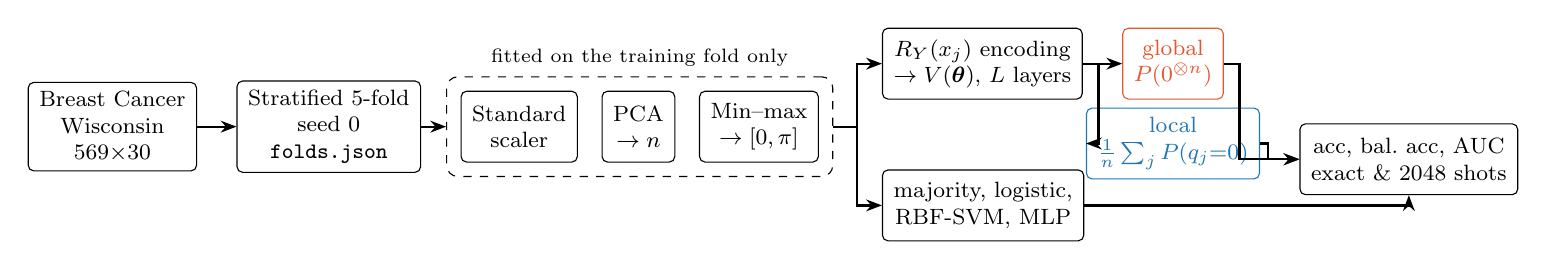
\begin{tikzpicture}[
  node distance=4mm and 5mm,
  box/.style={draw, rounded corners=2pt, align=center, font=\footnotesize,
              minimum height=9mm, inner xsep=4pt, fill=white},
  arr/.style={-{Stealth[length=2mm]}, thick}]
\node[box] (data) {Breast Cancer\\Wisconsin\\569$\times$30};
\node[box, right=of data] (folds) {Stratified 5-fold\\seed 0\\\texttt{folds.json}};
\node[box, right=of folds] (std) {Standard\\scaler};
\node[box, right=3mm of std] (pca) {PCA\\$\to n$};
\node[box, right=3mm of pca] (mm) {Min--max\\$\to[0,\pi]$};
\begin{scope}[on background layer]
\node[draw, dashed, rounded corners, fit=(std)(pca)(mm), inner sep=5pt,
      label={[font=\scriptsize]above:fitted on the training fold only}] (prep) {};
\end{scope}
\node[box, right=8mm of mm, yshift=8mm] (enc) {$R_Y(x_j)$ encoding\\$\to V(\boldsymbol\theta)$, $L$ layers};
\node[box, right=of enc, draw=cglobal, text=cglobal] (pg) {global\\$P(0^{\otimes n})$};
\node[box, below=1mm of pg, draw=clocal, text=clocal] (pl) {local\\$\frac1n\sum_j P(q_j{=}0)$};
\node[box, right=8mm of mm, yshift=-10mm] (cls) {majority, logistic,\\RBF-SVM, MLP};
\node[box, right=of pl, yshift=-2mm] (met) {acc, bal.\ acc, AUC\\exact \& 2048 shots};
\draw[arr] (data) -- (folds);
\draw[arr] (folds) -- (prep);
\draw[arr] (prep.east) -- ++(3mm,0) |- (enc.west);
\draw[arr] (prep.east) -- ++(3mm,0) |- (cls.west);
\draw[arr] (enc) -- (pg);
\draw[arr] (enc.east) -- ++(2mm,0) |- (pl.west);
\draw[arr] (pg.east) -- ++(2mm,0) |- (met.west);
\draw[arr] (pl.east) -- ++(1mm,0) |- (met.west);
\draw[arr] (cls.east) -| (met.south);
\end{tikzpicture}}
\caption{Classification pipeline. Every model, quantum or classical, sees the
same folds and the same fold-wise preprocessed features. The global and local
quantum models share the circuit and differ only in the readout.}
\label{fig:pipeline}
\end{figure*}

\subsection{Noise and hardware}\label{sec:noise}
Noisy simulations use Qiskit Aer with depolarizing (unital) and amplitude-damping
(non-unital) channels, plus a noise model taken from an IBM fake backend. This
separates cost-induced from noise-induced flattening~\cite{wang2021,singkanipa2025}
and tests whether the local cost holds up better under non-unital noise~\cite{mele2026}.
On IBM hardware we estimate parameter-shift gradients at $n\in\{2,4,6\}$,
$L=\lceil\log_2 n\rceil$, with 30--50 random draws and 4096 shots, using
the same circuits for both costs, and report the shot-noise contribution
next to each measured variance.

\subsection{Software and reproducibility}
Python~3.14, NumPy~2.5, scikit-learn~1.9.1, Qiskit~2.5.1 and Qiskit
Aer~0.17.2. One seed constant (0) is used throughout, with repeat seeds spaced by
100. Every number and figure is produced by a script in
\texttt{experiments/} or \texttt{viz/}. Results are saved as CSV, and the
fold file and the test suite are part of the repository.

% =====================================================================
\section{Results}
% =====================================================================
\emph{To be written in Week~2.}

\bibliographystyle{IEEEtran}
\bibliography{refs}

\end{document}
